\documentclass[12pt]{article}
\usepackage[paperwidth=36in,paperheight=20in,margin=0.8in]{geometry}
\usepackage[utf8]{inputenc}
\usepackage[T1]{fontenc}
\usepackage{booktabs}
\usepackage[table]{xcolor}
\usepackage{multicol}
\usepackage{tikz}
\usepackage{hyperref}
\usepackage{amsmath}

\pagestyle{empty}
\setlength{\columnsep}{0.6in}
\setlength{\parskip}{0pt}
\setlength{\parindent}{0pt}

% Robinhood color palette
\definecolor{rhbg}{HTML}{191B1C}
\definecolor{rhcard}{HTML}{2A2C2E}
\definecolor{rhgreen}{HTML}{21CE99}
\definecolor{rhtext}{HTML}{FFFFFF}
\definecolor{rhsecondary}{HTML}{C3C5C8}
\definecolor{rhborder}{HTML}{3A3C3E}

\pagecolor{rhbg}
\color{rhtext}

\newcommand{\postersection}[1]{%
  \vspace{0.5em}
  \noindent
  \hspace*{-\leftskip}%
  \colorbox{rhgreen}{\parbox{\dimexpr\linewidth-\rightskip-2\fboxsep\relax}{\textcolor{rhbg}{\textbf{\LARGE #1}}}}\par
  \vspace{0.3em}
}

% Pipeline box style
\tikzset{
  pipebox/.style={
    draw=rhgreen, thick, fill=rhcard, rounded corners=5pt,
    minimum height=0.9in, text width=4.0in, align=center,
    font=\large, inner sep=4pt, text=rhtext
  },
  pipearrow/.style={
    ->, thick, rhgreen, >=stealth, shorten >=2pt, shorten <=1pt
  }
}

\arrayrulecolor{rhgreen}
\hypersetup{urlcolor=rhgreen}

\begin{document}

% ========== HEADER BANNER ==========
\begin{tikzpicture}[remember picture, overlay]
  \fill[rhgreen] (current page.north west) rectangle ([yshift=-2.5in]current page.north east);
  \node[anchor=center, text=rhbg, font=\fontsize{48}{54}\selectfont\bfseries]
    at ([yshift=-1.1in]current page.north) {Can Economic Data Predict the Stock Market?};
  \node[anchor=center, text=rhbg, font=\fontsize{24}{28}\selectfont\bfseries]
    at ([yshift=-2.0in]current page.north) {A Machine Learning Approach to S\&P~500 Forecasting};
  \node[anchor=north west, text=rhbg, font=\fontsize{16}{18}\selectfont\bfseries]
    at ([xshift=0.8in, yshift=-0.3in]current page.north west) {Jagat Brahma \quad\textbar\quad jpbrahma@stanford.edu};
  \node[anchor=north east, text=rhbg, font=\fontsize{16}{18}\selectfont\bfseries]
    at ([xshift=-0.8in, yshift=-0.3in]current page.north east) {CS 229 --- Stanford University};
\end{tikzpicture}

\vspace{2.2in}

% ========== PIPELINE DIAGRAM ==========
\noindent
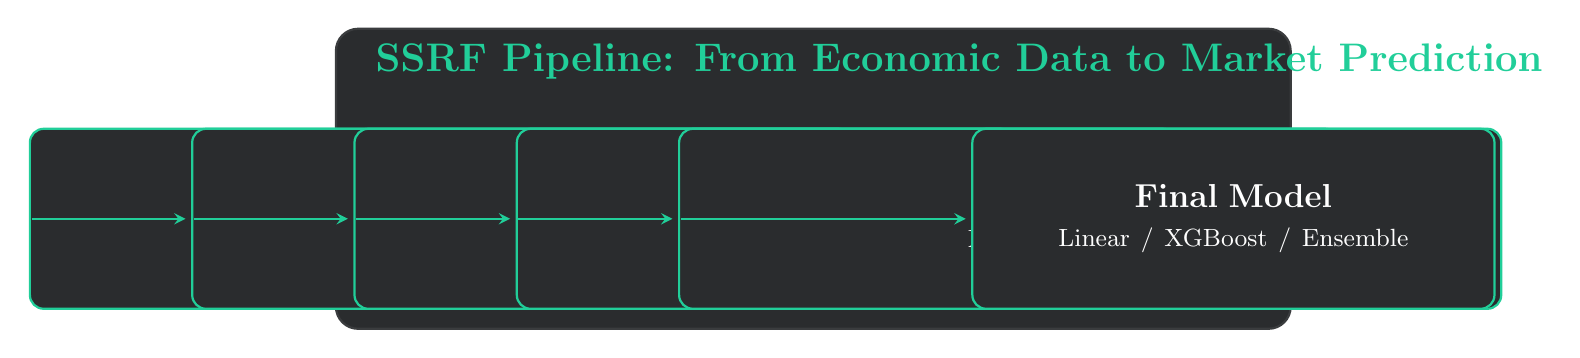
\begin{tikzpicture}
  \draw[rounded corners=8pt, fill=rhcard, draw=rhborder, thick]
    (0in, 0in) rectangle (\textwidth, 1.5in);
  \node[anchor=south west, text=rhgreen, font=\bfseries\Large]
    at (0.15in, 1.2in) {SSRF Pipeline: From Economic Data to Market Prediction};

  % Pipeline nodes
  \node[pipebox] (fred)  at (0.11\textwidth, 0.55in) {\textbf{FRED-MD Data}\\\small 134 monthly indicators};
  \node[pipebox] (s1)    at (0.28\textwidth, 0.55in) {\textbf{1. Screen}\\\small Keep best $\sim$50};
  \node[pipebox] (s2)    at (0.45\textwidth, 0.55in) {\textbf{2. Scale}\\\small Weight by predictive strength};
  \node[pipebox] (s3)    at (0.62\textwidth, 0.55in) {\textbf{3. PCA Factors}\\\small Compress to 10};
  \node[pipebox] (s4)    at (0.79\textwidth, 0.55in) {\textbf{4. Regime}\\\small Multiply by volatility};
  \node[pipebox, text width=2.5in] (pred) at (0.94\textwidth, 0.55in)
      {\textbf{Final Model}\\\small Linear / XGBoost / Ensemble};

  % Arrows
  \draw[pipearrow] (fred) -- (s1);
  \draw[pipearrow] (s1)   -- (s2);
  \draw[pipearrow] (s2)   -- (s3);
  \draw[pipearrow] (s3)   -- (s4);
  \draw[pipearrow] (s4)   -- (pred);
\end{tikzpicture}

\vspace{0.3in}

% ========== CONTENT BACKGROUND BOX ==========
\begin{tikzpicture}[remember picture, overlay]
  \draw[rounded corners=12pt, fill=rhcard, draw=rhborder, thick]
    ([xshift=0.8in, yshift=-4.8in]current page.north west)
    rectangle ++(34.4in, -13in);
\end{tikzpicture}

% ========== THREE-COLUMN LAYOUT ==========
\begin{multicols}{3}
\setlength{\leftskip}{0.3in}%
\setlength{\rightskip}{0.3in}%

% --- PREDICTING ---
\postersection{What We Built}

\large
We built a pipeline that reads \textbf{130+ monthly economic statistics}
(jobs, inflation, housing, interest rates) and predicts whether the
S\&P~500 will go up or down. We tested two horizons: next-month and
next-quarter forecasts, simulating real-time trading over 26 years.

% --- DATA ---
\postersection{Data}

\large
\textbf{Input:} 134 monthly economic indicators from the Federal Reserve's
FRED-MD database (1979--2026). Covers employment, industrial production,
housing, retail sales, interest rates, inflation, and consumer sentiment.

\textbf{Target:} S\&P~500 index returns from Yahoo Finance. Two targets:
(1) next month's return, and (2) cumulative return over the next 3 months.

\textbf{Size:} 540 months, 134 features. Training starts with 120 months
(10 years) and expands walk-forward --- no future data leaks in.

% --- FEATURES ---
\postersection{Features}

\large
Raw indicators are noisy and highly correlated. We process them in three
steps before feeding them to any model:
\begin{enumerate}
  \setlength\itemsep{0.2em}
  \item \textbf{Group-wise Screen} --- Each indicator gets a t-statistic
        measuring how well it predicts returns on its own. Within each
        economic category, we keep only the ones that show some signal.
        For example, of 20 interest-rate indicators (3-month T-bill,
        10-year yield, corporate spreads, etc.), only the strongest
        few survive. Same for jobs, inflation, housing --- preventing
        any single category from flooding the model with noise.
        Typically 40--60 indicators remain.
  \item \textbf{Predictive Scaling} --- Each surviving indicator is
        multiplied by how strongly it has historically predicted returns.
        For example, if the unemployment rate has been a strong predictor,
        it gets amplified; if housing starts have been a weak one, it
        gets shrunk. This way the next step focuses on what actually
        matters for forecasting.
  \item \textbf{Factor Extraction (PCA)} --- The remaining indicators
        still move together (they all track the same economy). Principal
        Component Analysis compresses them into 10 uncorrelated
        ``economic factors'' --- e.g., all employment indicators combine
        into a single labor factor, all interest rates into a rates
        factor, all inflation measures into a prices factor.
\end{enumerate}

We also create \textbf{regime interaction terms} --- multiplying each factor
by recent market volatility --- so the model adapts to calm vs.\ turbulent
markets.

\columnbreak

% --- MODELS ---
\postersection{Models}

\large
Seven models tested on the same pipeline:
\vspace{0.3em}

\noindent
\hspace*{-\leftskip}%
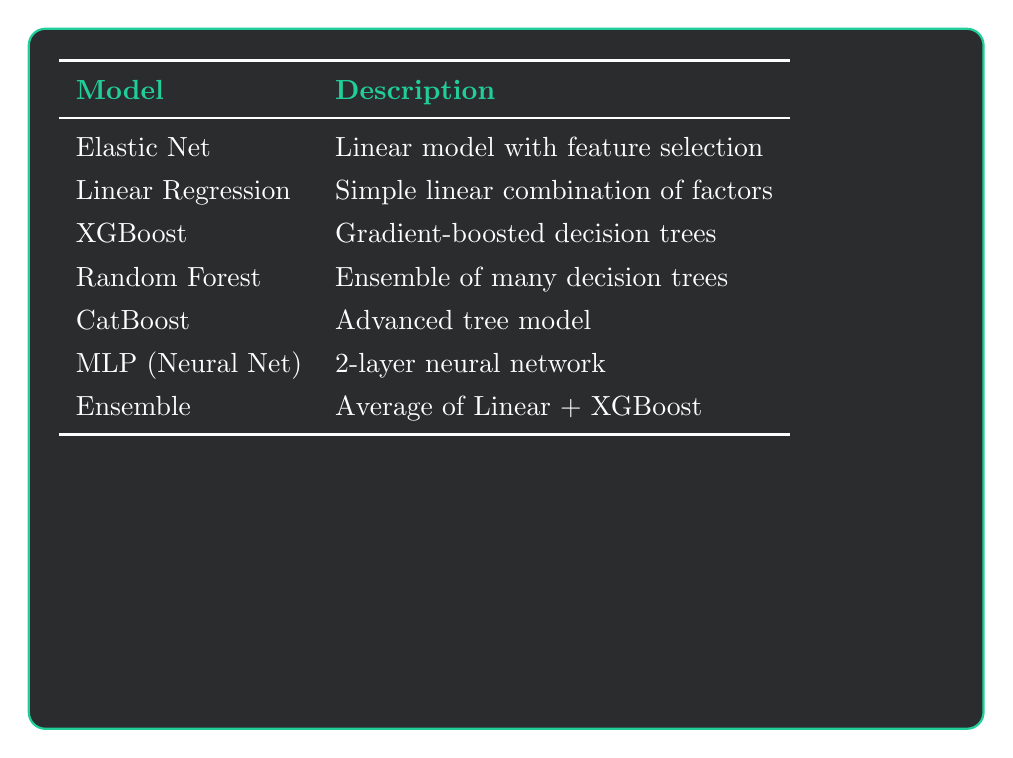
\begin{tikzpicture}
  \draw[rounded corners=6pt, fill=rhcard, draw=rhgreen, thick]
    (0,0) rectangle (\linewidth-\rightskip, 3.5in);
  \node[anchor=north west, text=rhtext, inner sep=0.15in]
    at (0,3.5in) {\parbox{\dimexpr\linewidth-\rightskip-0.3in\relax}{
      \renewcommand{\arraystretch}{1.3}
      \begin{tabular}{ll}
      \toprule
      \color{rhgreen}\textbf{Model} & \color{rhgreen}\textbf{Description} \\
      \midrule
      Elastic Net & Linear model with feature selection \\
      Linear Regression & Simple linear combination of factors \\
      XGBoost & Gradient-boosted decision trees \\
      Random Forest & Ensemble of many decision trees \\
      CatBoost & Advanced tree model \\
      MLP (Neural Net) & 2-layer neural network \\
      Ensemble & Average of Linear + XGBoost \\
      \bottomrule
      \end{tabular}
    }};
\end{tikzpicture}

\vspace{0.5em}
\textbf{Baselines:} Always-long (predict market always goes up) and
momentum (predict same direction as last month).

% --- RESULTS ---
\postersection{Results}

\large
\noindent
\hspace*{-\leftskip}%
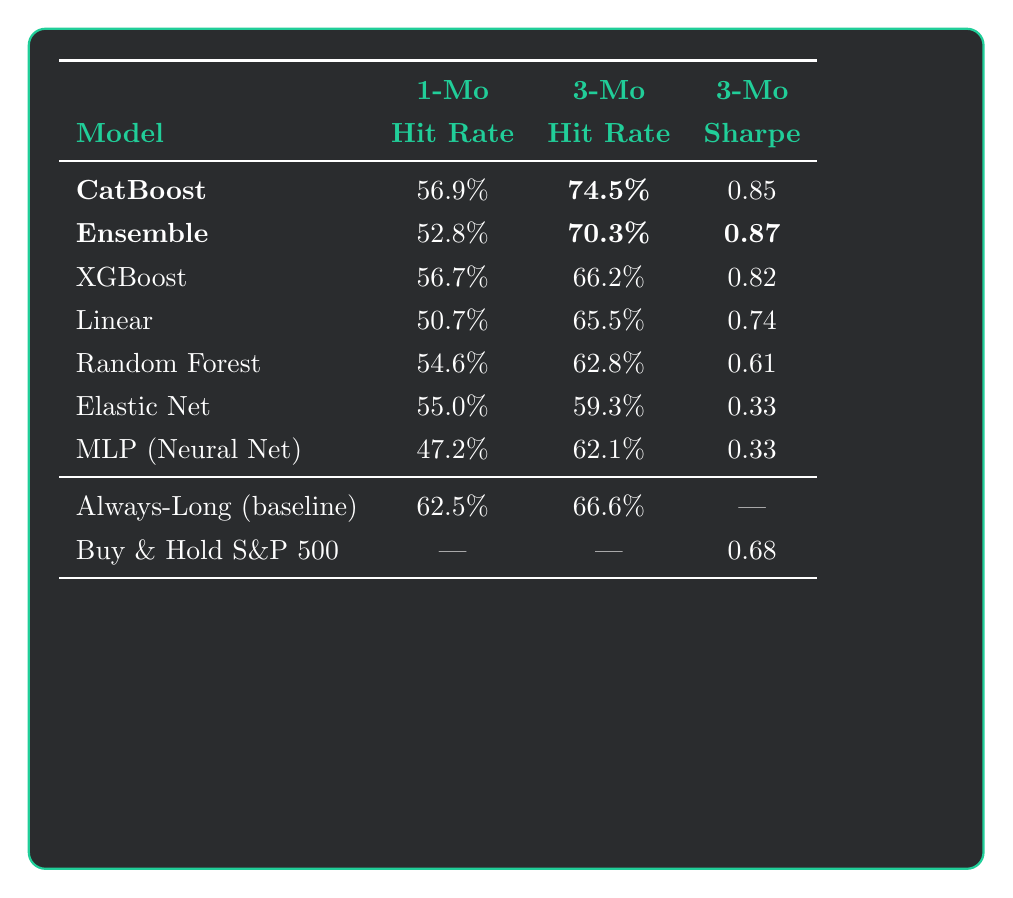
\begin{tikzpicture}
  \draw[rounded corners=6pt, fill=rhcard, draw=rhgreen, thick]
    (0,0) rectangle (\linewidth-\rightskip, 4.2in);
  \node[anchor=north west, text=rhtext, inner sep=0.15in]
    at (0,4.2in) {\parbox{\dimexpr\linewidth-\rightskip-0.3in\relax}{
      \renewcommand{\arraystretch}{1.3}
      \begin{tabular}{lccc}
      \toprule
      \color{rhgreen} & \color{rhgreen}\textbf{1-Mo} & \color{rhgreen}\textbf{3-Mo} & \color{rhgreen}\textbf{3-Mo} \\
      \color{rhgreen}\textbf{Model} & \color{rhgreen}\textbf{Hit Rate} & \color{rhgreen}\textbf{Hit Rate} & \color{rhgreen}\textbf{Sharpe} \\
      \midrule
      \textbf{CatBoost} & 56.9\% & \textbf{74.5\%} & 0.85 \\
      \textbf{Ensemble} & 52.8\% & \textbf{70.3\%} & \textbf{0.87} \\
      XGBoost & 56.7\% & 66.2\% & 0.82 \\
      Linear & 50.7\% & 65.5\% & 0.74 \\
      Random Forest & 54.6\% & 62.8\% & 0.61 \\
      Elastic Net & 55.0\% & 59.3\% & 0.33 \\
      MLP (Neural Net) & 47.2\% & 62.1\% & 0.33 \\
      \midrule
      Always-Long (baseline) & 62.5\% & 66.6\% & --- \\
      Buy \& Hold S\&P~500 & --- & --- & 0.68 \\
      \bottomrule
      \end{tabular}
    }};
\end{tikzpicture}

\vspace{0.8em}
\hspace*{-\leftskip}%
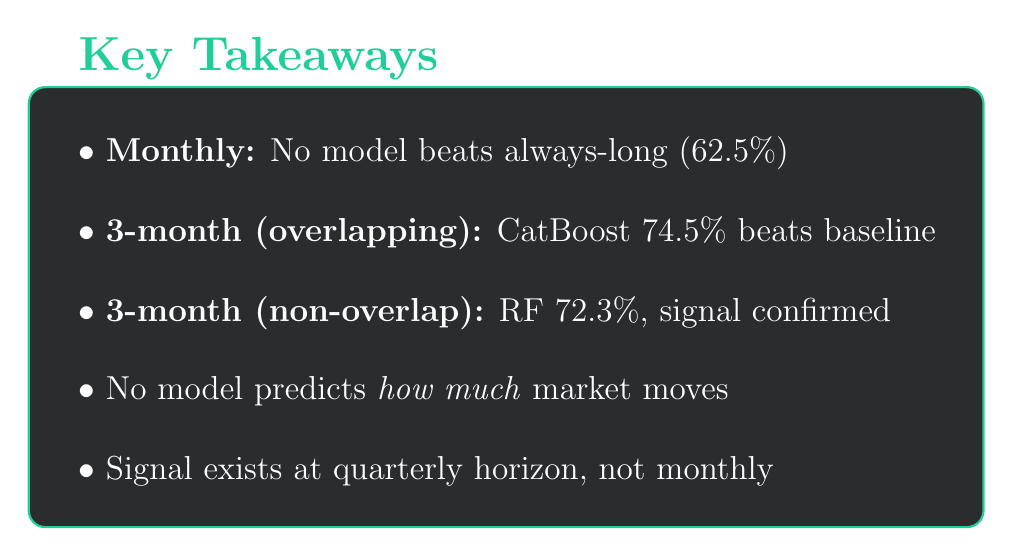
\begin{tikzpicture}
  \draw[rounded corners=6pt, fill=rhcard, draw=rhgreen, thick]
    (0,0) rectangle (\linewidth-\rightskip, 2.2in);
  \node[anchor=north west, text=rhgreen, font=\bfseries\LARGE]
    at (0.2in, 2.5in) {Key Takeaways};
  \node[anchor=north west, text=rhtext, font=\large]
    at (0.2in, 2.0in) {$\bullet$ \textbf{Monthly:} No model beats always-long (62.5\%)};
  \node[anchor=north west, text=rhtext, font=\large]
    at (0.2in, 1.6in) {$\bullet$ \textbf{3-month (overlapping):} CatBoost 74.5\% beats baseline};
  \node[anchor=north west, text=rhtext, font=\large]
    at (0.2in, 1.2in) {$\bullet$ \textbf{3-month (non-overlap):} RF 72.3\%, signal confirmed};
  \node[anchor=north west, text=rhtext, font=\large]
    at (0.2in, 0.8in) {$\bullet$ No model predicts \textit{how much} market moves};
  \node[anchor=north west, text=rhtext, font=\large]
    at (0.2in, 0.4in) {$\bullet$ Signal exists at quarterly horizon, not monthly};
\end{tikzpicture}

\columnbreak

% --- DISCUSSION ---
\postersection{Discussion}

\large
\textbf{Monthly:} All models fail. None beat the simple strategy of always
predicting up (62.5\% accuracy). This matches the well-known result that
next-month stock returns are unpredictable from economic data.

\textbf{Quarterly:} Real signal appears. CatBoost (74.5\%) beats the 66.6\%
baseline by nearly 8 points. The Ensemble reaches 70.3\% with the best
risk-adjusted return (Sharpe 0.87).

\textbf{But the signal is weak.} Models get \textit{direction} right but
can't predict \textit{magnitude}. All have negative $R^2_{OOS}$, meaning a
simple historical average predicts magnitudes better.

\textbf{Non-overlapping evaluation confirms signal.} Using independent quarterly
observations ({\tt --non-overlap} flag), Random Forest achieves 72.3\% hit
ratio and MLP a 0.84 Sharpe -- confirming direction signal is not an artifact
of overlapping windows.

\textbf{Leverage helps manage risk.} Asymmetric sizing (2.5$\times$ long,
0.25$\times$ short) cuts maximum loss from $\sim$47\% (buy \& hold) to
$\sim$10\%, though it slightly reduces Sharpe for the strongest models.

% --- WHAT DIDN'T WORK ---
\postersection{What Didn't Work}

\large
\begin{itemize}
  \setlength\itemsep{0.2em}
  \item \textbf{Extreme leverage} (25$\times$): destroyed all portfolios
  \item \textbf{Monthly returns}: hopeless at this horizon
  \item \textbf{Magnitude prediction}: all $R^2_{OOS}$ negative
  \item \textbf{Transaction costs}: eat 1--2\% of annual returns
\end{itemize}

% --- FUTURE WORK ---
\postersection{Future Work}

\large
\begin{enumerate}
  \setlength\itemsep{0.2em}
  \item Model actual release lags of economic data (FRED reports come weeks
        after month-end)
  \item Replace volatility proxy with a Hidden Markov Model for better
        regime detection
  \item Full transaction cost modeling for production systems
\end{enumerate}

% --- REFERENCES ---
\postersection{References}

\large
\begin{tabular}{ll}
{[1]} & Goyal \& Welch (2008). A Comprehensive Look. \\
{[2]} & Campbell \& Thompson (2008). Predicting Excess Returns. \\
{[3]} & McCracken \& Ng (2016). FRED-MD Database. \\
{[4]} & Zou \& Hastie (2005). Elastic Net. \\
\end{tabular}

\vspace{0.8em}
\begin{center}
\colorbox{rhcard}{\parbox{0.8\columnwidth}{\centering\large
\textbf{Code:} \url{https://github.com/pellucide/sp500\_macro\_forecast-}}}
\end{center}

\end{multicols}

\end{document}
